\documentclass[10pt,twocolumn]{article}
\usepackage{tikz}
\usetikzlibrary{positioning, arrows.meta, calc}
\usepackage{caption}

\begin{document}

\begin{figure*}[h!]
\centering
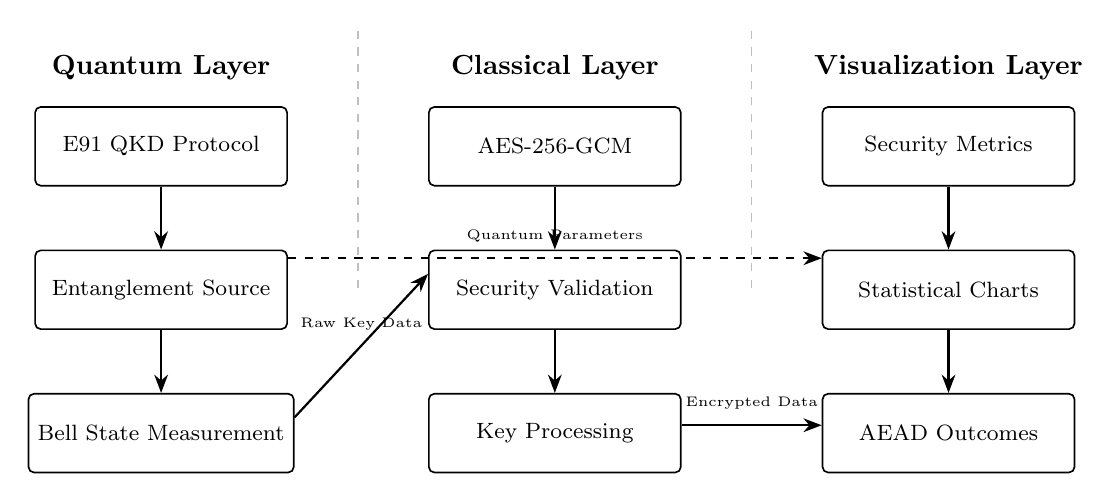
\begin{tikzpicture}[
    node distance=2.2cm and 3.5cm,
    every node/.style={font=\footnotesize},
    module/.style={
        rectangle,
        draw=black,
        fill=white,
        minimum width=3.2cm,
        minimum height=1cm,
        align=center,
        line width=0.6pt,
        rounded corners=2pt
    },
    title/.style={
        rectangle,
        fill=white,
        minimum width=3.2cm,
        minimum height=0.6cm,
        align=center,
        font=\bfseries
    },
    arrow/.style={
        -Stealth,
        line width=0.8pt,
        color=black
    }
]

% Quantum Layer
\node[title] (qtitle) at (0,4) {Quantum Layer};
\node[module] (e91) at (0,3) {E91 QKD Protocol};
\node[module, below=0.8cm of e91] (entangle) {Entanglement Source};
\node[module, below=0.8cm of entangle] (measure) {Bell State Measurement};

% Classical Layer
\node[title] (ctitle) at (5,4) {Classical Layer};
\node[module] (aes) at (5,3) {AES-256-GCM};
\node[module, below=0.8cm of aes] (validation) {Security Validation};
\node[module, below=0.8cm of validation] (processing) {Key Processing};

% Visualization Layer
\node[title] (vtitle) at (10,4) {Visualization Layer};
\node[module] (metrics) at (10,3) {Security Metrics};
\node[module, below=0.8cm of metrics] (charts) {Statistical Charts};
\node[module, below=0.8cm of charts] (results) {AEAD Outcomes};

% Horizontal Data Flow - Different heights for each arrow
\draw[arrow] ($(measure.east)+(0,0.2)$) -- ($(validation.west)+(0,0.2)$)
    node[midway, above, font=\tiny, yshift=2pt] {Raw Key Data};
    
\draw[arrow] ($(processing.east)+(0,0.1)$) -- ($(results.west)+(0,0.1)$)
    node[midway, above, font=\tiny, yshift=2pt] {Encrypted Data};

\draw[arrow, dashed] ($(entangle.east)+(0,0.4)$) -- ($(charts.west)+(0,0.4)$)
    node[midway, above, font=\tiny, yshift=2pt] {Quantum Parameters};

% Internal vertical connections
\draw[arrow] (e91.south) -- (entangle.north);
\draw[arrow] (entangle.south) -- (measure.north);
\draw[arrow] (aes.south) -- (validation.north);
\draw[arrow] (validation.south) -- (processing.north);
\draw[arrow] (metrics.south) -- (charts.north);
\draw[arrow] (charts.south) -- (results.north);

% Layer separation lines
\draw[dashed, gray!50, line width=0.4pt] (2.5,1.2) -- (2.5,4.5);
\draw[dashed, gray!50, line width=0.4pt] (7.5,1.2) -- (7.5,4.5);

\end{tikzpicture}

\caption*{Figure: Three-layer architecture of the hybrid quantum-classical cryptographic simulator.}
\label{fig:three_layer_architecture}
\end{figure*}

\end{document}